%\documentclass[a4paper,12pt]{report}
\documentclass[aps,prb,epsf,epsfig,floatfix,showpacs,groupedaddres,superscriptaddress]{revtex4-1}
%\documentclass[aps,prb,epsf,epsfig,floatfix,showpacs,groupedaddres,superscriptaddress,twocolumn]{revtex4-1}
%
%
%
\usepackage{amsmath, amssymb, txfonts, bm, graphicx, subcaption, float}
\usepackage{anysize}
\usepackage[margin=1in]{geometry}
%
%\usepackage{mycommand}
%\marginsize{3cm}{2cm}{1cm}{1cm}
%\usepackage{amssymb, txfonts}
%\usepackage{amsmath, bm}
%\usepackage{psfig}
%\usepackage{graphicx}
%\usepackage{epstopdf}
%\usepackage{amsxtra}
%%\usepackage{tikz}
%%\usepackage{subfigure}
%\usepackage{caption} 
%\usepackage{subcaption, float}
%\usepackage{multicol}
%%\usepackage{natbib}
%\usepackage{multirow}
%%\usepackage{newunicodechar}
%%\usepackage[dvips]{epsfig} 
%\usepackage{appendix}
\numberwithin{equation}{section}
%\newunicodechar{✓}{\checkmark}
\linespread{1.2}
\usepackage{algorithm,algorithmic}
%\usepackage{url}
%
\newtheorem{definition}{Definition}
\newtheorem{remark}{\textbf{Remark}}
\newtheorem{problem}{Problem}
\newtheorem{motivation}{Motivation}
\newtheorem{assumption}{\textbf{Assumption}}
\newtheorem{lemma}{\textbf{Lemma}}
\newtheorem{theorem}{\textbf{Theorem}}
\newtheorem{proposition}{Proposition}
\usepackage{makecell}
\usepackage{listings}
% user defined commands
%\newtheorem{theorem}{Theorem}
%\newtheorem{remark}{Remark} 
%\newtheorem{corollary}{Corollary}
%\newtheorem{lemma}{Lemma}
%\newtheorem{assum}{Assumption}
%\newtheorem{proof}{Proof}
\newcommand{\ubar}[1]{\text{\b{$#1$}}}
\newcommand{\bb}[1]{\varmathbb{#1}}
\newcommand{\norm}[1]{\left\lVert#1\right\rVert}
\newcommand{\abs}[1]{\left\lvert#1\right\rvert}
\newcommand{\at}[2][]{#1|_{#2}}
\newcommand\numberthis{\addtocounter{equation}{1}\tag{\theequation}}
\DeclareMathOperator{\sinc}{sinc}
\DeclareMathOperator*{\argmin}{arg\,min}
\setlength{\parindent}{0pt}
%\usepackage{xcolor}
\usepackage[usenames,dvipsnames,svgnames,table]{xcolor}
\usepackage{pstricks}
\definecolor{Blue}{rgb}{0.0,0.0,1.0} % Blue for keywords
\definecolor{Green}{rgb}{0.0,0.5,0.0} % Green for comments
\definecolor{Red}{rgb}{0.6,0.1,0.1} % Dark red for strings
\definecolor{backcolour}{rgb}{0.95,0.95,0.92}
%\definecolor{blue}{rgb}{1,0.75,0.8}
\newrgbcolor{dgreen}{0.0 0.4 0.0}
\newrgbcolor{pink}{1.0 0.0 0.4}
\newrgbcolor{violet}{0.6 0.0 0.4}
\newrgbcolor{orange}{1.0 0.2 0.0}
\newrgbcolor{dred}{0.8 0.1 0.0}
\usepackage{verbatim}
\usepackage{hyperref}
\hypersetup{
     colorlinks=true,
     citecolor=blue,
     urlcolor=violet,
     linkcolor=dgreen
}
\usepackage{empheq}
%%%%% Equation numbering --->
%\def\theequation{\thesection.\arabic{equation}}
\renewcommand{\theequation}{\arabic{equation}}
%
\lstdefinestyle{PythonStyle}{
    language=Python,
    basicstyle=\ttfamily\footnotesize,
     backgroundcolor=\color{backcolour},
     keywordstyle=\color{Blue},
     commentstyle=\color{Green},
     stringstyle=\color{Red},
     breaklines=true,
     numbers=left,
    %numberstyle=\tiny\color{gray},
    stepnumber=1,
    frame=single,
    showspaces=false,
    showstringspaces=false,
    showtabs=false,
    tabsize=4,
    captionpos=b,
    breaklines=true,
    breakatwhitespace=true
     % Enable line wrapping
    % Other style settings
}
\def\FIGDIR{FIGS_MANUS_NHSE}
\def\NHHMDIR{/Users/dirac/Documents/My_Talks/FIGS_NHHM}
%
\def\CT{\textcolor{red}{[citation needed!!]}}
%
\def\blgn#1\elgn{\begin{align}#1\end{align}}
\newcommand{\y}{^\dag}
\let\py\relax
\providecommand{\py}{^{\phantom \dag}}
\newcommand{\f}{\frac}
\def\h{\hat}
\def\al{\alpha}
\def\del{\delta}
\def\g{\gamma}
\def\l{\lambda}
\def\sig{\sigma}
\def\Om{\Omega}
\newcommand{\dv}{{\bf d}}
\newcommand{\kv}{{\bf k}}
\newcommand{\Av}{{\bf A}}
% Derivatives
\newcommand{\grad}{\nabla}
\newcommand{\curl}{{\nabla\times}}
\newcommand{\pd}{{\partial}}
\newcommand{\pdk}{{\partial_k}}
% Factors/Coeffcient
\newcommand{\fres}{2\pi i}
\newcommand{\finvtwpi}{\f{1}{2\pi}}
\newcommand{\finvres}{\frac{1}{2\pi i}}


% Blackboard 1
\usepackage{bbm}
\newcommand{\bbone}{\mathbbm 1} 
%
\newcommand{\Tr}{\text{Tr}} % Trace
\newcommand{\tr}{\text{tr}} % Trace
\def\tbs{[\textcolor{red}{*to be shown}]}
\newcommand{\mc}{\mathcal}
\newcommand{\mcC}{{\mc C}}
\newcommand{\mcF}{{\mc F}}
\newcommand{\mcS}{{\mc S}}
\newcommand{\bbmat}{\begin{bmatrix}}
\newcommand{\ebmat}{\end{bmatrix}}
\def\non{\nonumber}
\newcommand{\hc}{\text{h.c.}}
\newcommand{\bs}{\boldsymbol}
\newcommand{\eref}[1]{Eq. (\ref{#1})}
\newcommand{\erefs}[1]{Eq.s (\ref{#1})}
\newcommand{\lngl}{\langle}
\newcommand{\rngl}{\rangle}
\newcommand{\nk}{n,{\bf k}}
\newcommand{\inv}{{^{-1}}}
\def\pd{\partial}
\def\bi{\begin{itemize}}
\def\ei{\end{itemize}}
\def\i{\item}
\newcommand{\bnu}{\begin{enumerate}}
\newcommand{\enu}{\end{enumerate}}
\def\Ra{\Rightarrow}
%
\def\p#1{\blue{#1}}  % paint text
\def\alert#1{\textcolor{red}{#1}}  % text in red
%% Footnote
\newcommand\blfootnote[1]{%
  \begingroup
  \renewcommand\thefootnote{}\footnote{#1}%
  \addtocounter{footnote}{-1}%
  \endgroup
}
%
\renewcommand{\thefootnote}{$\dag$}
\newcommand{\rbul}[2][darkred,fill=darkred]{\tikz[baseline=-0.5ex]\draw[#1,radius=#2] (0,0) circle ;}%
%\def\rb{\rbul{2pt} \hspace{0.5cm}}
\def\rb{\rbul{2pt}~}
\def\ralert#1{\rb\alert{#1}}
%
\def\tp{t_+}
\def\tm{t_-}
\def\etal{\emph{et al.}}
%%% ------------------------  DOCUMENT BEGINS -----------------------------------------------
\begin{document}

\title{Non-Hermitian Skin Effect: A Primer}
\author{Sagnik Seth}\email{sag123nik456@gmail.com}
\affiliation{IISER Kolkata, Kolkata, India}
%
\author{Bihan Bhowmick}\email{bihan.bhowmick@students.iiserpune.ac.in}
\affiliation{IISER Pune, Pune, India}
%
%
\author{Himadri Barman}\email{reducedpc@gmail.com}
\affiliation{Department of Physics, Zhejiang University, Hangzhou 310027, China}
%
\begin{abstract}
Hermiticity is a crucial condition for the observables to be real (hence measuarble) 
in our conventional quantum physics.
However, the conventional quantum physics deals with the ideal scenario where the system
is isolated from its environment. As soon as we take account of the interaction with the 
environment, we enter the generic world of non-equilibrium quantum physics where Hermiticity
is not a required condition. The recent hunt of topological insulators for fault-tolerant 
quantum computation has opened the gate for studying the physics of non-Hermiticity into
those materials. It has been recently discovered that non-Hermiticity induces an exotic
phenomenon dubbed the \emph{skin effect} which entails asymmetric localization of 
quantum states. In our article, we provide an introduction to this phenomenon and physics
behind this with a flavor of students-friendly pedagogy.    
\end{abstract}
\maketitle

%\newpage
\def\hHN{{\hat H}_{\rm{HN}} }
\def\hSSH{{\hat H}_{\rm{SSH}} }
\def\hNHSSH{{\hat H}_{\rm{NHSSH}} }
\tableofcontents

\newpage
\section{Introduction}

\section{Hatano-Nelson model: A flavor of non-Hermiticity in a lattice}
The Hatano-Nelson model (non-disordered) is the simplest tight-binding
lattice model where the left and right-moving hopping amplitudes are unequal
(\emph{non-reciprocal}). The Hamiltonian for spinless particles in one dimension reads
\blgn
 \hHN = \sum_{i=0}^{L-1} \big[t_R c\y_i c\py_{i+1} + t_L c\y_{i+1} c\py_i \big]\,,   
\elgn
where $L$ is the lattice size; $t_R$ and $t_L$ are the right and left hopping
amplitudes; $c\py_i$ and  $c\y_i$ are the particle anihilation and
creation operators at lattice site $i$, respectively.

We can express the anihilation operator in terms of Fourier components as
\blgn
c_{i}\equiv \f{1}{\sqrt L}\sum_{k=0}^{L-1} e^{ik.x_i} c_{k}.
\elgn 
(where $x_i$ is the coordinate or position of site $i$)
and rewrite the Hamilotonian in the Fourier ($k$) space:
\blgn
 \hHN &= \sum_{i=0}^{L-1}\sum_{k=0}^{L-1}\sum_{k'=0}^{L-1} 
     \big[t_R c\y_k c\py_k e^{ik'((x_{i+1}-kx_i)} + t_L c\y_k c\py_k e^{ik'(x_{i}-kx_{i+1}} \big]\non\\
     &=\sum_i\sum_k\big[t_R c\y_k c\py_k e^{ik((x_{i+1}-x_i)} + t_L c\y_k c\py_k e^{i(x_{i}-x_{i+1}} \big]
      \quad\mbox{[Dropped details of summantion indices for clarity]}\non\\
     &=\big[t_R e^{ika} + t_L e^{-ika}\big]c\y_k c\py_k 
\elgn
where we utilize $x_{i+1}-x_i=a$, $a$ being the lattice constant (spacing between two consecutive lattice sites).
%% FIG: HN chain
\begin{figure}[!htp]
\centering
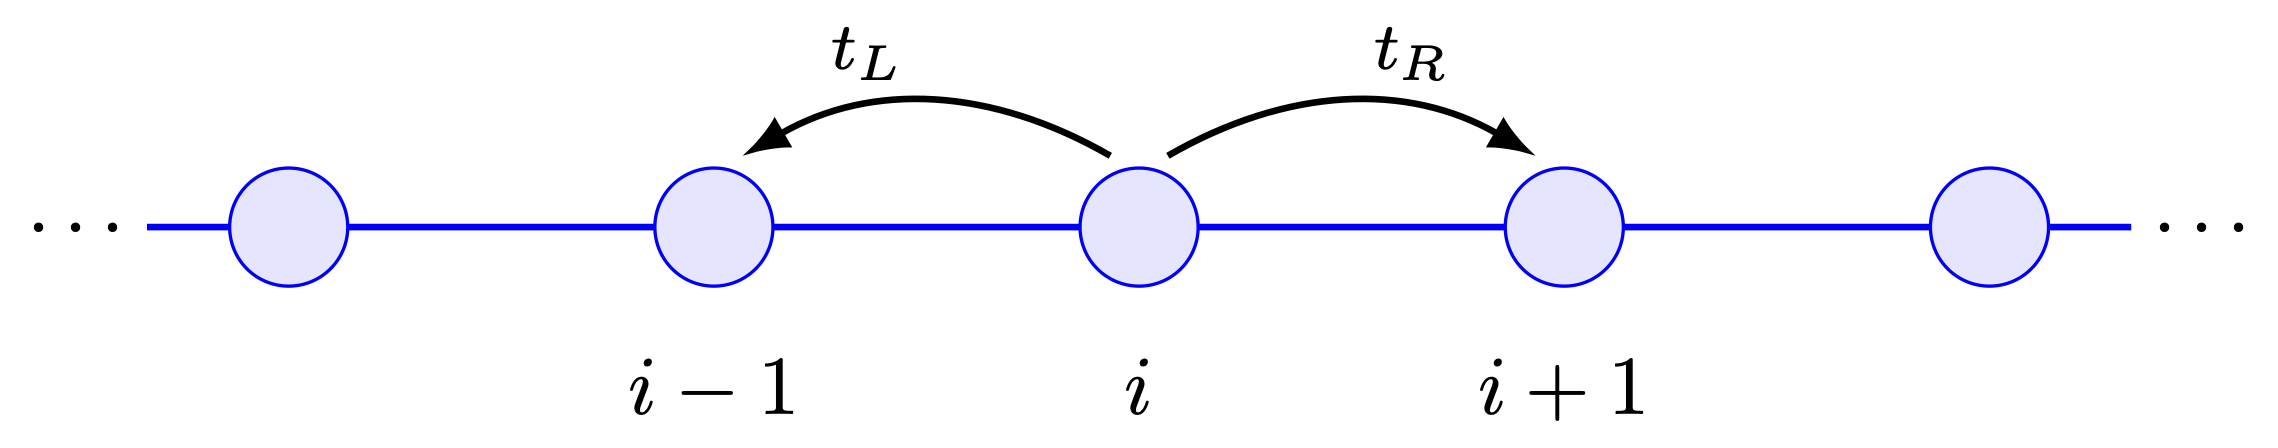
\includegraphics[height=1.5cm,clip]{\FIGDIR/HNchain.png}
\caption{Hatano-Nelson chain with non-reciprocal hopping parameters $t_R$ and $t_L$.}
\end{figure}


\section{SSH model}
Let us start with the simplest topological model Hamiltonian known 
as the Su-Schrieffer-Heeger (SSH) model
which has been used to describe polyacetylene or bi-partite/dimerized (Peierls) lattice
~\cite{su:schrieffer:heeger:prl79}.
%[Barisic et al, 1970, Su et al 1979]. 
The Hamiltonian reads
%
\blgn
\hSSH
&=\sum_{I=1}^{L} [t+(-1)^I\del]c\y_I c\py_{I+1}\non\\
&=\sum_{i=0}^{L-1} (t+\del )c\y_{A\,i} c\py_{B\,i} + \sum_i (t-\del )c\y_{A\,i+1} c\py_{B\,i}+\hc\,\non\\
&\equiv \sum_i [\tp c\y_{A\,i} c\py_{B\,i} + \tm c\y_{A\,i+1} c\py_{B\,i}+\hc]\,.
\label{eq:H:SSH:ispace}
\elgn
Here the lattice consists of two different sublattice sites $A$ and $B$
inside each primitive cell as they associate with two different hopping amplitudes, namely 
$\tm = t-\del$  (representing longer single bond having lesser kinetic energy or hopping for $\del>0$) and $\tp = t + \del$ (representing shorter double bond having higher kinetic energy or hopping for $\del>0$). $\tp$ and $\tm$ are dubbed \emph{intracell} and \emph{intercell} hopping respectively.
%% FIG: SSH chain
\begin{figure}[!htp]
\centering
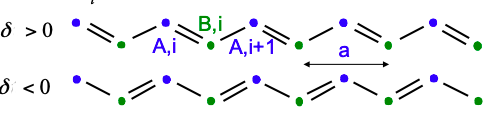
\includegraphics[height=1.5cm,clip]{\FIGDIR/SSH_chains.png}
\caption{Su-Schrieffer-Heeger (SSH) chains in two different configurations.}
\end{figure}



Now the Hamiltonian can be written in the matrix
form $\h H= {\bs\Psi}\y {\bf H}  {\bs\Psi}$ with the basis (or spinor)
$\bs{\Psi}\y=[ c\y_{A\,1} c\y_{B\,1} c\y_{A\,2}\cdots ]$. Then the Hamiltonian matrix becomes
\blgn
{\bf H}
=
\bbmat
0      &\tp    &0      &\cdots    &0\\
\tp^*    &0      &\tm  &\cdots   &0\\
\vdots &\vdots &\vdots &\vdots     &0\\
0      &0      &0      &t_{L-1}^*   &0
\ebmat
\elgn
where the $(L-1)$-th hopping amplitude 
$t_{L-1}$ is either $\tp$ or $\tm$ depending on the value of $L$ (even or odd).\\
Note that the above matrix represents the open boundary condition (OBC) where there
exists no left-side hopping from cell 1 (considering cell 2 is on the right of cell 1) and no right-side hopping  from cell $L$. 
However, if the periodic boundary condition (PBC) is applied, i.e. 
left-side hopping from cell 1 is the last cell $L$ and right-side 
hopping from cell $L$ finds the cell 1 back, then the Hamiltonian becomes 
\blgn
{\bf H}
=
\bbmat
0      &\tp    &0      &\cdots &t_L^*\\
\tp^*    &0      &\tm    &\cdots &0\\
\vdots &\vdots &\vdots &\vdots &0\\
t_L      &0      &0      &t_{L-1}  &0
\ebmat
\elgn

To see a demonstration, take a simple example of a 4-site (2-cell) lattice (two $A$-sites + two $B$-sites) with OBC:
\blgn
{\bf H}_{4\times 4}
=
\bbmat
0       &\tp     &0       &0\\
\tp^*   &0       &\tm     &0\\
0       &\tm^*   &0       &\tp\\
0       &0       &\tp^*   &0
\ebmat
\elgn

Then 
\blgn
\h H_{4\times 4}
&= \Psi\y {\bf H}_{4\times 4} \Psi\non\\
&=\bbmat
c\y_{A1} &c\y_{B1} &c\y_{A2} &c\y_{B2}
\ebmat
\bbmat
0       &\tp     &0       &0\\
\tp^*   &0       &\tm     &0\\
0       &\tm^*   &0       &\tp\\
0       &0       &\tp^*   &0
\ebmat
\bbmat
c\py_{A1} \\c\py_{B1} \\c\py_{A2} \\c\py_{B2}
\ebmat\non\\
%
&=\bbmat
c\y_{A1} &c\y_{B1} &c\y_{A2} &c\y_{B2}
\ebmat
\bbmat
\tp c\py_{B1} \\\tp^*c\py_{A1}+\tm c\py_{A2} \\\tm^*c\py_{B1}+\tp c\py_{B2} \\\tp^* c\py_{A2}
\ebmat\non\\
%
&=
\tp c\y_{A1}c\py_{B1} 
+ \tp^* c\y_{B1}c\py_{A1} + \tm c\y_{B1}c\py_{A2}\non\\ 
&\quad + \tm^*c\y_{A2}c\py_{B1} + \tp c\y_{A2}c\py_{B2}
+\tp^* c\y_{B2} c\py_{A2}\,.
\elgn


\section{Reciprocal space representation}
\def\tc{\tilde{c}}
Now we want to write the Hamiltonian in the reciprocal ($k$) space. 
Again we can define the Fourier component of an annihilation operator:
\blgn
c_{\al k}\equiv \f{1}{\sqrt L}\sum_{i=1}^L e^{-ik.x_i} c_{\al i};\quad \al=A,B\,.
\elgn
[ Note: We have total $2L$ lattice sites consisting of $L$ number of $A$ and $B$ sublattices.]

Considering lattice coordinate at site $i$ to be $x_i$ with lattice spacing
$a$ (i.e., nearest neighbor site's position $x_{i+1}=x_i+a$), we can rewrite the Hamiltonian
in \eref{eq:H:SSH:ispace}: 
\blgn
\h H 
&= \sum_i \sum_{kk'}\bigg[\bigg\{\tp  c\y_{Ak}c\py_{Bk}e^{ik x_i}e^{-ik' x_i} + \hc\bigg\}\non\\
&\quad+\bigg\{\tm c\y_{Ak}c\py_{Bk}e^{ik(x_i+a)}e^{-ik' x_i} + \hc\bigg\}\bigg]\non\\
%%
&= \sum_{kk'}\bigg[\bigg\{\tp  c\y_{Ak}c\py_{Bk}\del_{kk'} + \hc\bigg\}\non\\
&\quad+\bigg\{\tm c\y_{Ak}c\py_{Bk}\del_{kk'} e^{-ik' x_i} + \hc\bigg\}\bigg]\non\\
&\qquad\qquad\quad\mbox{[use $\sum_i e^{i(k-k')x_i}=\del_{kk'}$]}\non\\
%%
&=\sum_k[\{\tp c\y_{Ak}c\py_{Bk}+ \tp^* c\y_{Bk}c\py_{Ak}\}\non\\
&\quad+\{\tm c\y_{Ak}c\py_{Bk}e^{-ik a} + \tm^*c\y_{Bk}c\py_{Ak} e^{ika}\}]\non\\
&\equiv \sum_k H_k\,.
\elgn

Thus we get the momentum ($k$) dependent Hamiltonian (for simplicity, we consider the hopping parameters to be real, i.e. $\tp^*=\tp$, $\tm^*=\tm$)
\blgn
H_k
&=\tp (c\y_{Ak}c\py_{Bk}+ c\y_{Bk}c\py_{Ak})
+\tm (c\y_{Ak}c\py_{Bk}e^{-ik a} + c\y_{Bk}c\py_{Ak} e^{ika})\\
&=(\tp+\tm e^{-ik a})c\y_{Ak}c\py_{Bk} + (\tp+\tm e^{ika}) c\y_{Bk}c\py_{Ak}\,.
\label{eq:Hk:SSH:matrix}
\elgn

Like what we did in the direct lattice representation case, we choose a 2-dimensional spinor
${\bs\Psi\y_k}\equiv [c\y_{Ak}\, c\py_{Bk}]$ and write $H_k$ in a $2\times2$ matrix form: 
$H_k={\bs\Psi\y_k}{\bf H}_k{\bs\Psi_k}$
where
\blgn
{\bf H}_k
\equiv
\bbmat
0 & \tp+\tm e^{-ika}\\
\tp+\tm e^{ika} & 0
\ebmat\,.
\elgn

Then \eref{eq:Hk:SSH:matrix} can be written in the following form:
\blgn
{\bf H}_k=d_x {\bs\sig}_x + d_y {\bs\sig}_y={\vec d}(k).{\vec\sig}\,
\label{eq:Hk:SSH:compact}
\elgn
where $d_x(k)\equiv\tp+\tm\cos ka$, $d_y(k)\equiv \tm \sin ka$; ${\bs\sig}_x=\bbmat 0 &1\\ 1 &0\ebmat$ 
and  ${\bs\sig}_y=\bbmat 0 &-i\\ i &0\ebmat$.


\section{Digression: Berry phase}
The Bloch wave function is not unique: $|u_\kv\rngl\to e^{i\phi(\kv)}|u_\nk\rngl$ is invariant under the gauge transformation $\Av \to \Av +\grad_\kv \phi(\kv)$ where
\blgn
\Av=i\lngl u_\kv|\grad_\kv u_\kv\rngl
\elgn
is known as the \emph{Berry connection} (analogous to the magnetic vector potential). 
For any close loop $\mcC$ in the $\kv$-space, the Berry phase can be defined as
\blgn
\gamma_C=\oint_\mcC \Av.d\kv =\int_\mcS \mcF d^2\kv\,
\elgn 
where $\mcF\equiv \curl A$ is known as the \emph{Berry curvature}.

For a TLS Hamiltonian $H(\kv)=\vec{d}(\kv).\vec{\sig}$, Berry showed~\cite{berry:prs84}\tbs
\blgn
\g_\mcC=\Om/2
\elgn
where $\Om$ is the solid angle swept out by $\h d(\kv)$.

\def\Qe{Q_\text{end}}
%\def\Qe{Q_\text{e}}


\section{Digression: Two level system}
In general a two-level Hamiltonian can be written as
\blgn
\h H_0=E_1|1\rngl\lngl 1| + E_2 |2\rngl\lngl 2|\,
\elgn
The Hamiltonian in the matrix form becomes
\blgn
H_0 =
\bbmat
E_1 &0\\
0   &E_2
\ebmat
\elgn

Now if we turn on an interaction $V$ between state $|1\rngl$ and $|2\rngl$,
we get an interacting Hamiltonian
\blgn
\h H=E_1|1\rngl\lngl 1| + E_2 |2\rngl\lngl 2| + V|1\rngl\lngl 2| + V^*|2\rngl\lngl 1|\,
\elgn
which gets the matrix form
\blgn
{\bf H}=
\bbmat
E_1 &V\\
V^*   &E_2
\ebmat
\elgn

The eigenvalue equation becomes
\blgn
(E_1-E)(E_2-E)-|V|^2=0
\elgn
which yields two eigenvalues $E_+$ and $E_-$ given by
\blgn
E_\pm=(E_1+E_2)\pm\sqrt{(E_1-E_2)^2+4|V|^2}\,.
\elgn

Suppose we have the following Hamiltonian
\blgn
{\bf H}(k)
=
\bbmat
h_0+h_z  &h_x-ih_y\\
h_x+ih_y &h_0-h_z
\ebmat
\elgn

Then the Hamiltonian can be written as
\blgn
H(k)=h^\mu(k)\sig_\mu=h_0(k)\bbone + \vec{h}(k).\vec{\sig}\,
\elgn
where $\bbone$ is the $2\times2$ unity matrix.

With $\Tr(H)=2h_0$ and $\det (H)=h_0^2-h^2$, one finds the eigenvalues
\blgn
E_\pm=h_0\pm h(k)
\label{eq:dispersion:tls}
\elgn
where 
\blgn
h(k)=||\vec{h}(k)||=\sqrt{h_x^2+h_y^2+h_z^2}\,.
\elgn
The corresponding normalized eigenvectors are (up to a phase factor)
\blgn
u_\pm(k)
=\f{1}{\sqrt{1+(h_z+E_\pm^2)/(h_x^2+h_y^2)}}
\bbmat
E_\pm/(h_x+ih_y)\\
1
\ebmat\,.
\elgn


\section{Back to the SSH model}
\subsection*{Dispersion:}
Now if we compare our $k$-space SSH Hamiltonian in 
\eref{eq:Hk:SSH:compact}, we notice 
$h_0$ and $\vec{h}(k) = \vec{d}(k)$. Therefore
from \eref{eq:dispersion:tls}
\blgn
E_k
&=\pm |\dv(k)|=\pm\sqrt{(t_+ + t_-\cos ka)^2+t_-^2\sin^2 ka}\label{eq:disp:SSH:1}\\
&=\pm \sqrt{(t_+ - t_-)^2+4t_+t_-\cos^2(ka/2)}\non\\
&=\pm \sqrt{(4 \del^2+4t_+t_-\cos^2(ka/2)}\,.
\label{eq:disp:SSH:2}
\elgn
with 
$d_x(k)\equiv\tp+\tm\cos ka$, $d_y(k)\equiv \tm \sin ka$.

\begin{comment}
\begin{figure}[!htp]
\centering
\includegraphics[height=1cm,clip]{\NHHMDIR/SSH_chain_Asboth.png}
%\caption{Su-Schrieffer-Heeger (SSH) chains in two different confi.}
\end{figure}
\end{comment}

\subsection*{Other Nomenclatures:}
In many literatures, the intracell hopping $\tp = t+\del$
is denoted by $v$ and intercell hopping $\tm = t-\del$
is denoted by $w$. Now onward, we shall follow this notation
and according to it,
\blgn
d_x(k) &\equiv v+w\cos ka; \quad d_y(k)\equiv w \sin ka\,
\label{eq:dx:dy:in:v:w}
\elgn
and
\blgn
E(k)=\pm\sqrt{v^2+w^2+2vw\cos ka}\,.\non
\elgn

From \eref{eq:dx:dy:in:v:w},
we get
\blgn
(d_x-v)^2 + d_y^2 &= w^2
\elgn
which describes a circle of radius $w$, centered at $(v,0)$.

%
\begin{figure}[!htp]:
\centering
\includegraphics[height=5cm,clip]{\NHHMDIR/SSH_dispersion_winding_no.png}
%\caption{Su-Schrieffer-Heeger (SSH) chains in two different confi.}
\end{figure}
\blfootnote{Courtesy: Asb\'oth \etal, \url{arXiv:1509.02295v1} }

\section{Winding number ($\nu$): The rubber band analogy} 
Winding number is a  many times a curve winds around a specific point $z_0$. 
\begin{figure}
	\centering\includegraphics[height=4cm,clip]{\NHHMDIR/Winding_Number_wiki.png}
\end{figure}

\alert{Our case:}
 $z_0 = (d_x=0,d_y=0)$ $\nu=1$ is {\blue topologically non-trivial!}
\begin{figure}
	\includegraphics[height=3cm,clip]{\NHHMDIR/delzero_winding.png}
	\includegraphics[height=3cm,clip]{\NHHMDIR/delposi_winding.png}
	\includegraphics[height=3cm,clip]{\NHHMDIR/delnegi_winding.png}
\end{figure}

The winding number can be mathematically formualated as
[{\red Check derivation!}]:
\blgn
\nu = \f{1}{2\pi} \int_{-\pi}^{\pi}dk\,\bigg( \h {\bf d}(k)\times \f{d}{dk}  \h {\bf d}(k)\bigg)_z\,.
\elgn
When the intracell hopping dominates over the intercell hopping (i.e. $v > w$), the winding number 
$\nu = 0$. On the other hand, when $v < w $, $\nu = 1$. to change $\nu$, we need to change the path 
of $\dv(k)$

\subsection*{Formula 4}
Since $E(k)=\pm|\dv(k)|$, we have
\blgn
 \ln E(k) &= \ln |\dv(k)| + i\arg(\dv(k))\,.\non\\
 \Ra \pdk \ln E(k) &= \pdk\ln |\dv(k)| + i\pdk\arg(\dv(k))\,.
\elgn

Now we know
\blgn
\nu = \finvtwpi \oint_C \pdk\arg(\dv(k)) \quad\mbox{[see above]}\,.  
\elgn

Also,
\blgn
\nu = \f{1}{2\pi i} \oint_C dk\, \pd_k \ln E_k\,. 
\elgn

Also,
\blgn
\nu = \f{i}{2\pi} \int_{C_\beta} dq\, q\inv. 
\elgn
 

\section{Edge states}
\alert{2 degenerate $E=0$ bands} 
\begin{figure}
	\includegraphics[height=3cm,clip]{\NHHMDIR/SSH_band_E_vs_v.png}
	\includegraphics[height=3cm,clip]{\NHHMDIR/SSH_modpsi_vs_site.png}
	\includegraphics[height=3cm,clip]{\NHHMDIR/SSH_barplot_edge1_vs_site.png}
	\includegraphics[height=3cm,clip]{\NHHMDIR/SSH_barplot_edge2_vs_site.png}
	\includegraphics[height=3cm,clip]{\NHHMDIR/SSH_barplot_bulk_vs_site.png}
\end{figure}
\bi
\i Edge states function as connectors/interfaces between 2 toplogical distinct phases
[trivial ($\nu=0$) and non-trivial ($\nu=1$)] $\Ra$ \blue{Bulk-boundary correspondence (BBC)}.
\ei

%\subsection*{References}
\bnu
 \i Shen: Topolgical Insulator and Dirac Equation in Condensed Matter
\i \url{http://optics.szfki.kfki.hu/~asboth/topins_course/2015-09-24-ELTE-Topins.pdf}
\i %\url{https://phyx.readthedocs.io/en/latest/TI/Lecture\%20notes/1.html}
 \enu



%% =================================================================================


\begin{comment}
\subsection*{Berry phase:}
The function $1+\cos ka\ge 0$ $\forall\,k$. Hence
when $\delt>0$, we always have $d_x(k)=t(1+\cos ka) +\delt\,(1-\cos ka)>0$.
Thus $d_x(k)$ sweeps no solid angle at $\delt>0$. On the other hand, 
when $\delt<0$,  $d_x(k)=2\delt$ at $k=\pm \pi/a$; this  $d_x(k)$ sweeps an angle
$2\pi$ {\red[more clear explanation needed, e.g. how it sweeps a solid angle]}.


\section{Polarization in 1D}
Electric polarization $\Pv$ is defined as the dipole moment per unit volume. 
Polarization leads to the bound charge $\rho_b=-\grad.\Pv$ in the bulk and 
surface/edge/end charge $\sig_b=\Pv.\ncap$ in 3D/2D/in. In the 1D we rename
the end charge as $\Qe$ and it simply becomes the magnitude of polarization
\blgn
\Qe=P\,.
\elgn
 
The polarization in 1D can be identified with the Berry phase 
of the occupied Bloch wavefunctions around the Brillouin zone:
\blgn
P=\f{e}{2\pi}\oint_\BZ A(k)dk\,.
\elgn
[{\bf N.B.} Detailed derivation is not straigh-forward, should be found in the literature.]\tbs


\section{Thouless charge pump}
  The integer charge pumped across a 1D insulator in one period of an adiabatic cycle
is a topological invariant that characterizes the cycle. (Courtesy: Kane's slide)

\blgn
H(k,t+T)=H(k,t)\,
\elgn
leads to
\blgn
\Del P=\f{e}{2\pi}\oint dk\, (A(k,T)-A(k,0)=ne\,,
\elgn
where
\blgn
n=%\f{1}{2\pi}\nint_{T^2} \Fv dk\,dt\,.
\elgn
\end{comment}


%\chapter{Non-Hermitian SSH}
\section{Non-Hermitian Topological Insulators} 

\alert{Hamiltonian in direct space}
\blgn
\h H &= B \sum_i (t_1-\gamma/2)\, c\y_{A\,i} c\py_{B\,i}
+ \sum_{i}(t_1+\gamma/2)\, c\y_{B\,i} c\py_{A\,i}\non\\
&\quad+ \sum_{i} t_2 \big[ c\y_{A\,i+1} c\py_{B\,i} +  c\y_{B\,i} c\py_{A\,i+1} \big]
+ \sum_{i}t_3 \big[c\y_{A\,i} c\py_{B\,i+1}+c\y_{B\,i+1} c\py_{A\,i}\big]\,.
\elgn
\begin{figure}
	\includegraphics[height=3cm,clip]{\NHHMDIR/Yao_Wang_NHSSH.png}
\end{figure}
\blfootnote{\dgreen{Yao and Wang, Phys. Rev. Lett., {\bf 121}, 086803 (2018)}}

\section{Exceptional points}
\alert{Complex eigenenergies}
\begin{figure}
	\includegraphics[height=3cm,clip]{\NHHMDIR/Yao_Wang_ModE_vs_t1_no_t3.png}
	\includegraphics[height=3cm,clip]{\NHHMDIR/Yao_Wang_ReE_vs_t1_no_t3.png}
	\includegraphics[height=3cm,clip]{\NHHMDIR/Yao_Wang_ImE_vs_t1_no_t3.png}
\end{figure}

\section{Edge states}
\alert{Edge states no longer symmetric}
\begin{figure}
	\includegraphics[height=3cm,clip]{\NHHMDIR/Yao_Wang_mod_edge_states_vs_site.png}
	\includegraphics[height=3cm,clip]{\NHHMDIR/Yao_Wang_barplot_edge1_vs_site.png}
	\includegraphics[height=3cm,clip]{\NHHMDIR/Yao_Wang_barplot_edge2_vs_site.png}
	\includegraphics[height=3cm,clip]{\NHHMDIR/Yao_Wang_barplot_bulk_vs_site.png}
\end{figure}
\bi
\i Even the bulk gets `edged': {\blue Non-Hermitian Skin Effect (NHSE)!} 
\ei

\section{Non-Bloch Band Theory}

\section{Project proposal}
\alert{Proposal A:}
\bi
\i Extensively study various non-Hermitian SSH models (for both diagonal and off-diagonal 
non-Hermiticity).
\i Add interaction to it (e.g. Hubbard type) and study.
\i Extend dimensionality and study.
\i Maybe design or perform an experiment.  
\ei
%
\alert{Proposal B:}
\bi
\i Extend the 2-site non-Hermitian problem to a lattice model. 
\i Employ sophisticated methods such as DMRG, MPS. 
\ei

\section*{References}
%\bibliographystyle{apsrev4-1}
%\bibliographystyle{prsty}
\bibliography{refs_nh}

\end{document}
